\documentclass[tikz,border=6pt]{standalone}
\usepackage{fontspec}
\usepackage{xeCJK}
\setmainfont{Times New Roman}
\setCJKmainfont{Hiragino Sans GB}
\setCJKsansfont{Microsoft YaHei}
\setCJKmonofont{STSong}
\usepackage{amsmath}
\usepackage{xcolor}
\usetikzlibrary{arrows.meta,positioning,calc}

\definecolor{srcgreen}{HTML}{2ECC71}
\definecolor{nodepurple}{HTML}{9B59B6}
\definecolor{sinkred}{HTML}{E74C3C}
\definecolor{edgegray}{HTML}{2C3E50}

\begin{document}
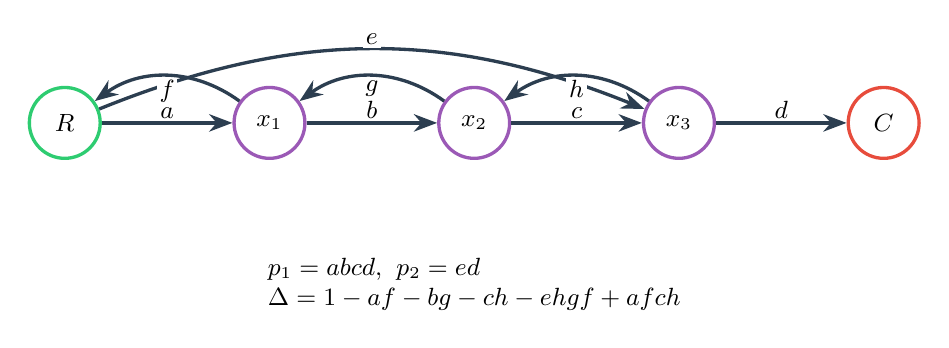
\begin{tikzpicture}[
  >=Stealth,
  line width=1.2pt,
  sfgsource/.style={circle, draw=srcgreen, minimum size=9mm, inner sep=0pt, font=\small\bfseries},
  sfgnode/.style={circle, draw=nodepurple, minimum size=9mm, inner sep=0pt, font=\small\bfseries},
  sfgsink/.style={circle, draw=sinkred, minimum size=9mm, inner sep=0pt, font=\small\bfseries},
  sfgedge/.style={->, draw=edgegray, line width=1.2pt},
  gaina/.style={font=\small\itshape, fill=white, inner sep=1pt}
]
  \node[sfgsource] (r) at (0,0) {$R$};
  \node[sfgnode] (x1) at (2.6,0) {$x_1$};
  \node[sfgnode] (x2) at (5.2,0) {$x_2$};
  \node[sfgnode] (x3) at (7.8,0) {$x_3$};
  \node[sfgsink] (c) at (10.4,0) {$C$};

  \draw[sfgedge] (r) -- node[gaina, above] {$a$} (x1);
  \draw[sfgedge] (x1) -- node[gaina, above] {$b$} (x2);
  \draw[sfgedge] (x2) -- node[gaina, above] {$c$} (x3);
  \draw[sfgedge] (x3) -- node[gaina, above] {$d$} (c);
  \draw[sfgedge, bend left=22] (r) to node[gaina, above] {$e$} (x3);

  \draw[sfgedge, bend right=36] (x1) to node[gaina, below] {$f$} (r);
  \draw[sfgedge, bend right=36] (x2) to node[gaina, below] {$g$} (x1);
  \draw[sfgedge, bend right=36] (x3) to node[gaina, below] {$h$} (x2);

  \node[font=\small\bfseries, align=left] at (5.2,-2.05) {$p_1=abcd,\ p_2=ed$\\$\Delta=1-af-bg-ch-ehgf+afch$};
\end{tikzpicture}
\end{document}
